\documentclass{article} % For LaTeX2e
\usepackage{nips13submit_e,times}
\usepackage{hyperref}
\usepackage{url}
\usepackage{graphicx}
%\documentstyle[nips13submit_09,times,art10]{article} % For LaTeX 2.09


\title{  Extracting and Aggregating Aspect-Level Sentiment from Product Reviews  }


\author{
Desmond C. Ong, Shane Soh, Matthew Long \\
Stanford University \\
\texttt{\{dco, shanesoh, mlong14\}@stanford.edu}
%Matthew Long \\
%Stanford University\\
%\texttt{mlong14} \\
%\And
%Desmond C. Ong \\
%%Psychology \\
%Stanford University \\
%\texttt{dco} \\
%\And
%Shane Soh \\
%%Affiliation \\
%Stanford University \\
%\texttt{shanesoh} \\
}

% The \author macro works with any number of authors. There are two commands
% used to separate the names and addresses of multiple authors: \And and \AND.
%
% Using \And between authors leaves it to \LaTeX{} to determine where to break
% the lines. Using \AND forces a linebreak at that point. So, if \LaTeX{}
% puts 3 of 4 authors names on the first line, and the last on the second
% line, try using \AND instead of \And before the third author name.

\newcommand{\fix}{\marginpar{FIX}}
\newcommand{\new}{\marginpar{NEW}}

\nipsfinalcopy % Uncomment for camera-ready version

\begin{document}


\maketitle

\begin{abstract}
Previous work in \textit{aspect-level sentiment analysis}---identifying the sentiment associated with products and their individual attributes, like battery life---have mostly been formulated as supervised learning problems, requiring known labels of both the relevant aspects and their sentiment. Here we propose a hybrid method where we first generate aspects from natural language text via unsupervised clustering of word vector representations, and secondly extract aspect-level sentiment. We then proceed to summarize these aspect-level sentiment within and across reviews and provide visualizations to aid consumers.
\end{abstract}

\section{Introduction}

In today's e-commercialized society, the consumer not only has access to online stores through which she might purchase anything she desires, but she also has unprecedented access to a deluge of information---most notably, product reviews written by other consumers---with which she can make her decision. Unfortunately, sifting through hundreds of reviews across tens of different websites to acquire specific information about the product and its important attributes (e.g. \textit{battery life}, \textit{screen size}, or \textit{weight} for electronics) is a time-consuming chore. It is difficult to automatically summarize this information, especially because of the heterogeneity of attributes across different product categories. Because of this, there has been much recent research tackling the two separate but interconnected components of this problem: (1) automatic discovery of aspects, and (2) aspect-specific sentiment analysis.

Within the context of a product review, the first component, \textit{aspect discovery}, involves identifying individual ``aspects" (which could be the product itself, or features/attributes of the product). This is made more difficult by the fact that relevant aspects might differ across similar products. For example, for a given electronic item such as a mobile phone, relevant aspects could be the battery life, screen size, weight, cost, and more. Not all these aspects are relevant across other electronic items: for a computer, weight might not be an issue, and screen size might be moot for headphones. 

The second component, \textit{aspect-specific sentiment analysis} involves subsequently identifying the sentiment---positive, neutral, or negative judgments---associated with aspects [1-6]. 

%Finally, The second problem involves aggregation of reviews, or constructing a \textit{meta-review}. Previous work [8-10] has shown that simple averaging of the ``stars" of reviews for an individual product is sub-optimal. Here we propose a deep learning architecture to aggregate the previously identified aspect-specific sentiment across multiple sentences within a review, and furthermore, to aggregate these sentiment across multiple reviews.





\section{Related work}

\textbf{Aspect Discovery}: Previous methods have used graphical models to attempt to extract 

Previous methods have relied on graphical models (e.g. Latent Dirichlet Allocation [1-3], or Conditional Random Fields [4]) to model latent aspects. We propose using similar unsupervised methods to generate candidate aspects via semantic word vector representations. 

In this paper, we propose extending recent successful advances in deep learning [6-7] to address this problem. In particular, we seek to improve and extend the work in [6], who used deep learning architectures like the Recursive Neural Tensor Network (RNTN) to extract aspect and sentiment in a single step. Unfortunately, supervised methods (e.g. [5-7]) that require labeled aspects-sentiment pairs for training are unscalable, and a better approach would be to automatically identify relevant aspects for each product (which, e.g. [1-3] try to do via topic modeling). 




\section{Approach}


\subsection{Aspect Discovery}

\textbf{Problem}: Given a short list of attributes (``seed" attributes), we discover an expanded list of attributes by returning the top $n$ related word vectors based on cosine similarity.



\subsection{Aspect-Specific Sentiment Extraction}



\begin{figure}[ht]
\begin{center}
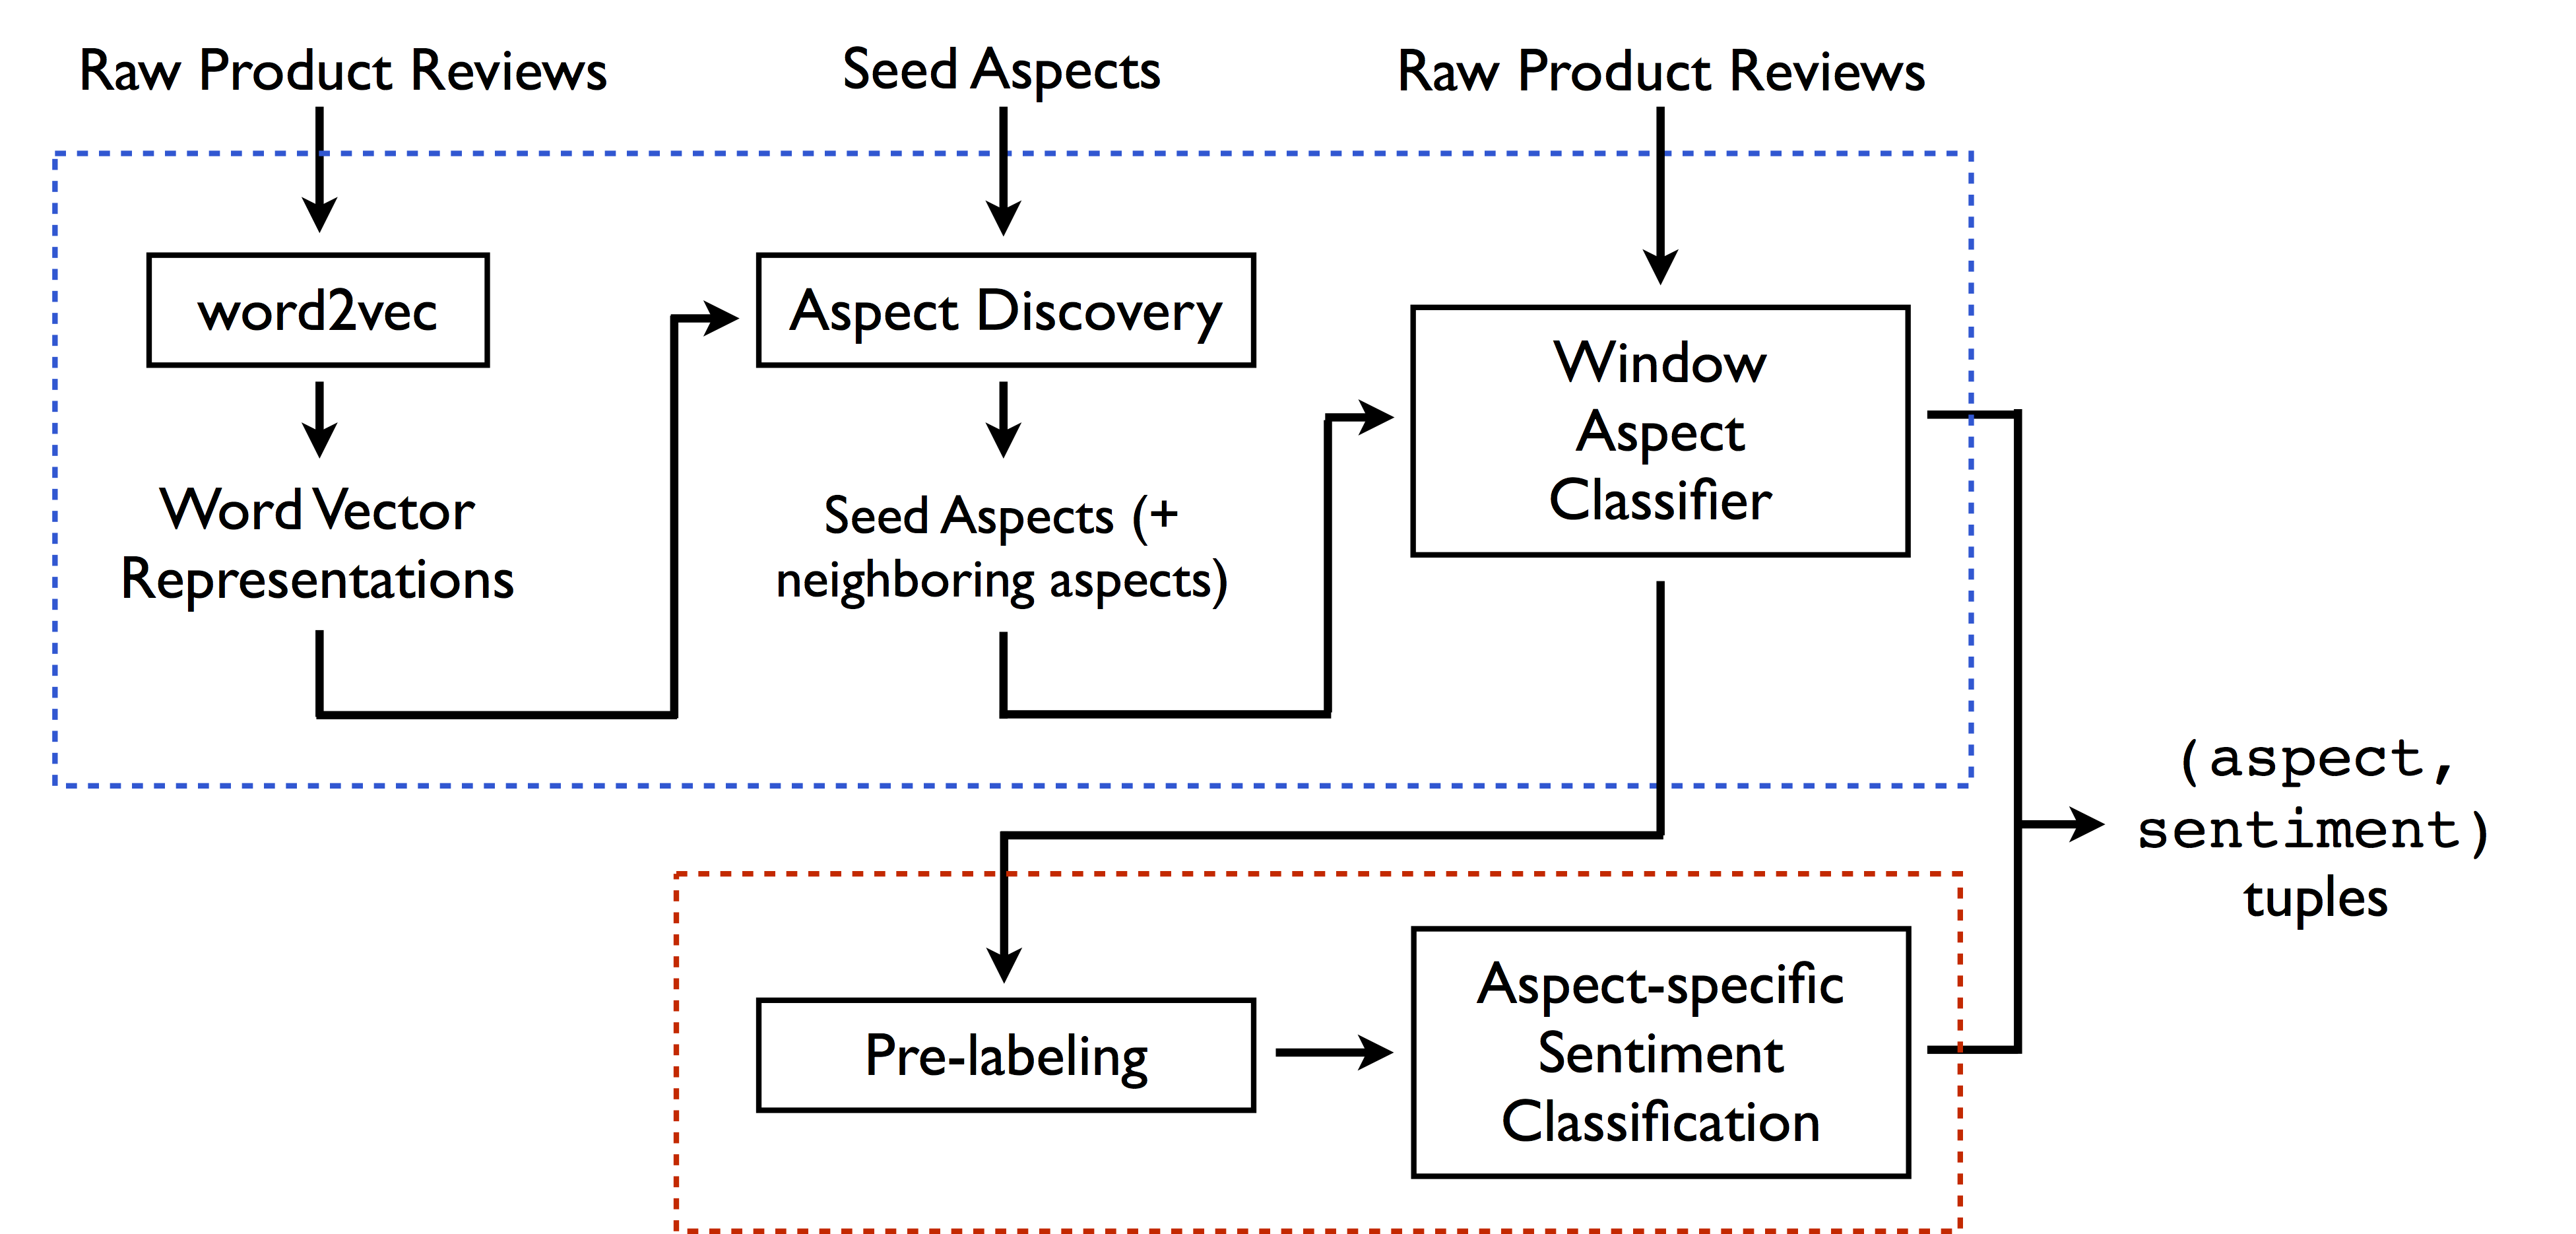
\includegraphics[width=.85\columnwidth]{workflow.png}
\end{center}
\caption{Proposed Workflow. Boxed items are processes, while non-boxed items are outputs. The left third of the diagram involves converting the reviews into a word vector representation, the middle third details unsupervised aspect discovery, while the right half of the diagram involves aspect-specific sentiment extraction, summarization and visualization.}% Except for the Sentiment Labeling and Visualization processes, every other process involves deep learning.}
\label{workflow}
\end{figure}

Our proposed workflow can be divided into two main parts: (unsupervised) {\bf Aspect Discovery} and {\bf Aspect-Specific Sentiment Extraction}. See Fig. \ref{workflow} for an illustration.

\textbf{Problem}: Given a set of product reviews (for a single product), identify (aspect, aspect-related sentiment) tuples. This is a similar problem statement as [6]: we intend to expand upon their model.

\textbf{Evaluation}: We will construct word cloud visualizations color coded to express sentiment. We will also perform comparisons with ``expert review" sites like CNET and DPReview (e.g. DPReview specifically rates digital cameras along certain chosen dimensions).

\begin{figure}[ht]
\begin{center}
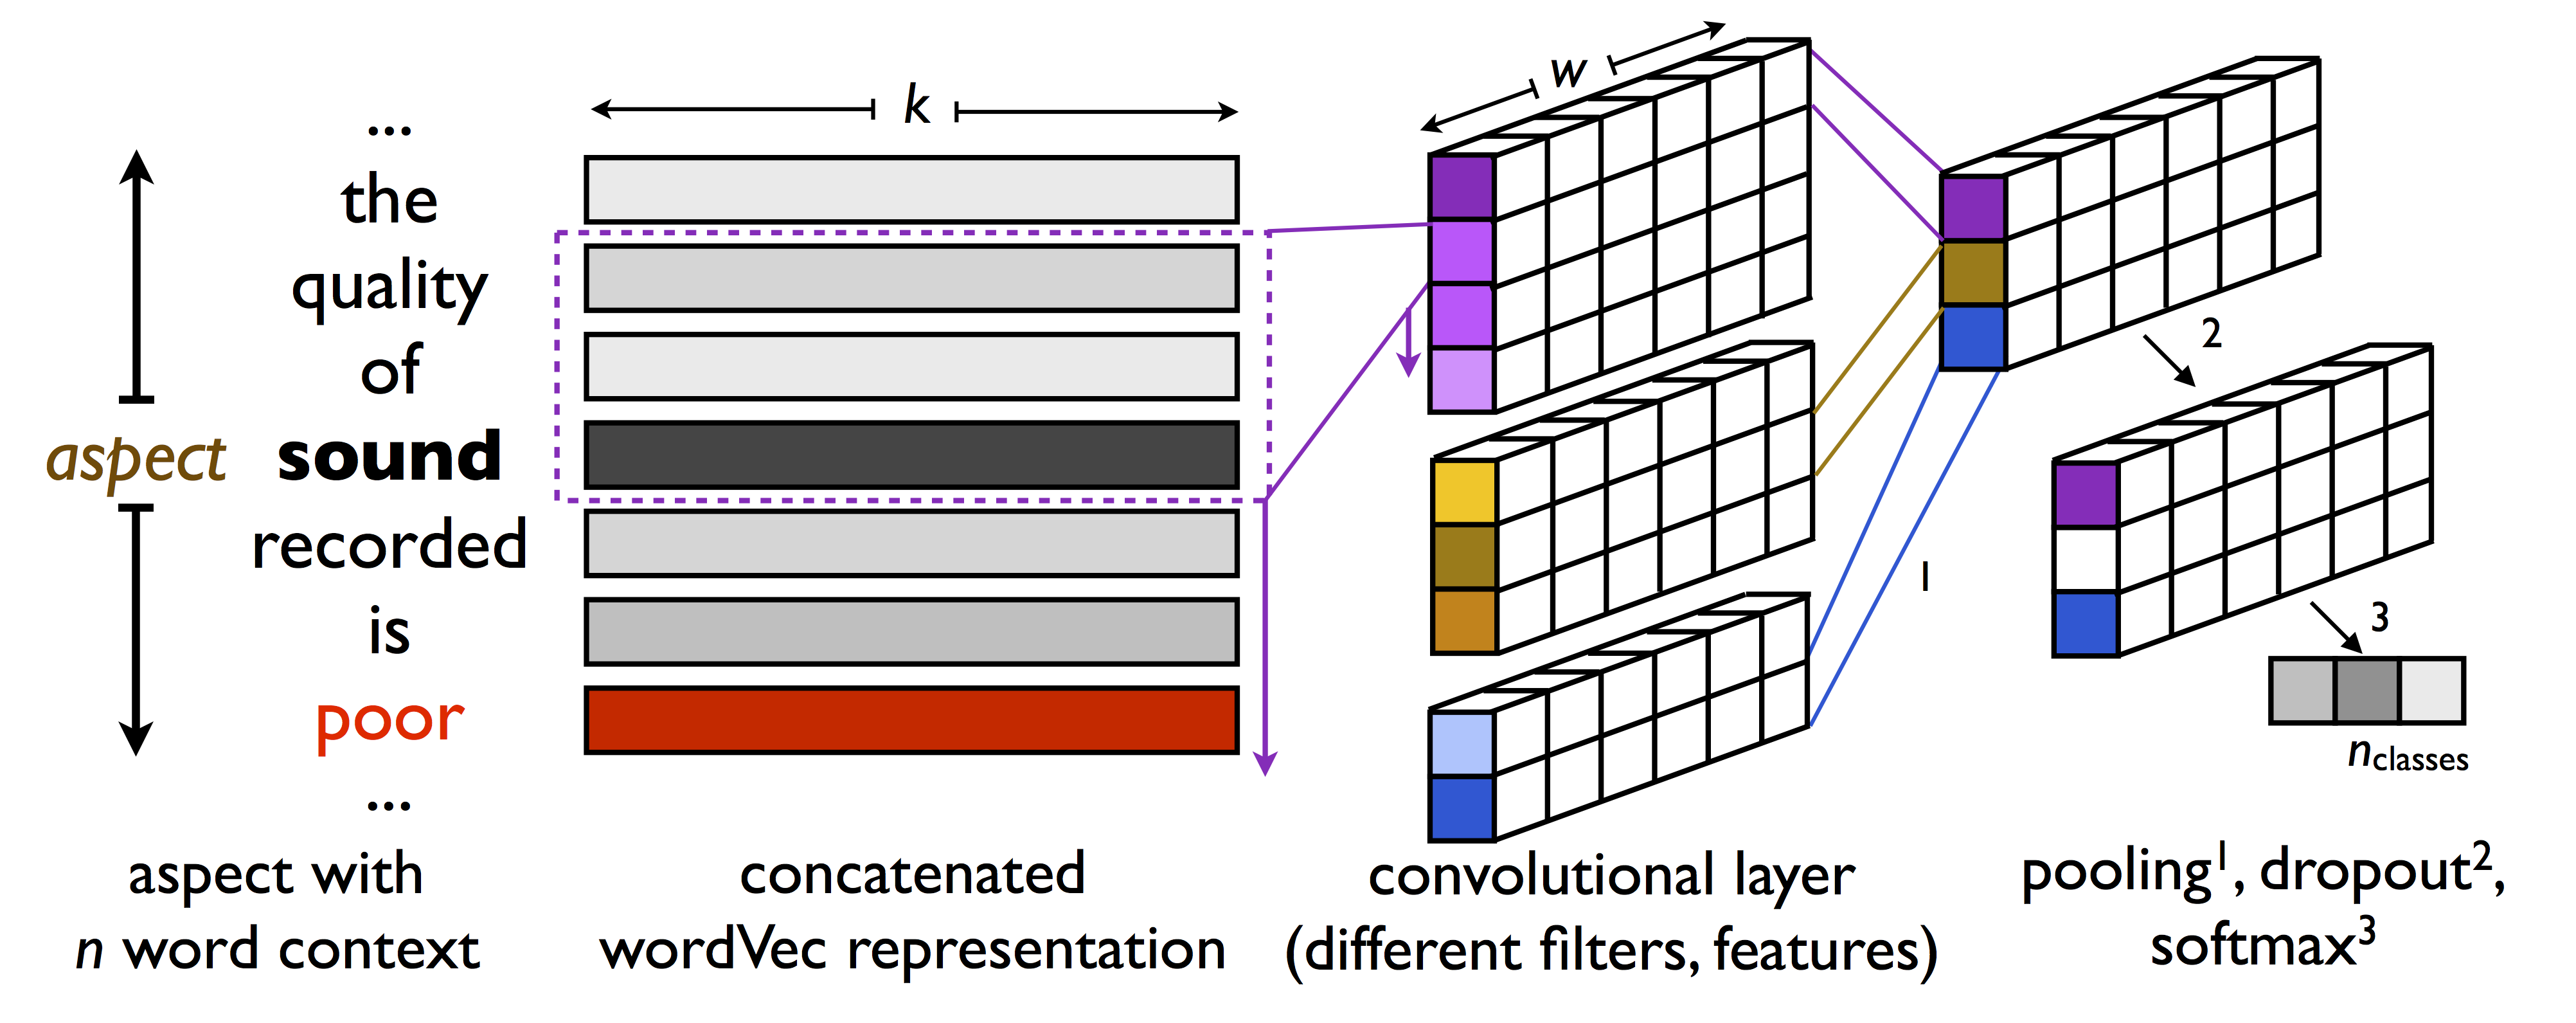
\includegraphics[width=.85\columnwidth]{model_architecture.png}
\end{center}
\caption{Model Architecture.}
\label{architecture}
\end{figure}


\section{Experiment} 

\textbf{Dataset}: 6 million reviews of electronic products from Amazon.com [8].



\subsection{Aspect Discovery}

The first part of the project involves an unsupervised approach to generating aspects. We tokenized our corpus using NLTK's punkt tokenizer [9] for sentence splitting. We then removed all non-alphanumerical characters and replaced all digits with \texttt{DG}. Finally, we performed collocation detection to detect common bigrams. We run word2vec (CBOW, Skipgram) to obtain a word vector representation of the data (varying hyper parameters like window size). We start with a list of seed attributes across a wide range of products, and discover more via closest cosine similarity.

\subsection{Aspect-Specific Sentiment Extraction}

An additional step would be to label all unigrams with a sentiment analysis lexicon (Bing Liu's sentiment lexicon) or the Sentiment pipeline in CoreNLP [7]. With the aspect-labels from the previous part, we would have a dataset labeled with aspect and (unigram-) sentiment. Next, we build off and improve on the model in [6]: we will use a RNTN or improved architecture to extract (aspect, aspect-specific sentiment) tuples from the data. Finally, we will have a summarization of aspect-related sentiment via visualization of our output, in terms of a word cloud of important aspects (e.g., sized by word frequency and colored by sentiment). 






\section{Results}

\subsection{Model Training} We trained three different word2vec models. The most successful model was trained using the CBOW (continuous bag-of-words) model with a window size of 10 and feature dimension size of 300. We also ignored all words with total frequency count below 40 (this helped to remove many typos). We determined the performance of each model by querying the model with various aspects common to electronic products (e.g. "portability", "screen quality", etc).

\subsection{word2vec Results}
We queried our word2vec model and returned the top-10 results based on cosine similarity of the word vectors.




%\begin{table}[h]
%\begin{center}
%\scalebox{0.7}{
%    \begin{tabular}{ | l | p{9cm} |}
%    \hline
%    Query & Results \\ \hline
%    \texttt{portability} & \texttt{(u'portability,', 0.72859996557235718), (u'compactness', 0.64743077754974365), (u'mobility', 0.60842603445053101), (u'versatility', 0.5763777494430542), (u'simplicity', 0.53962129354476929), (u'lightness', 0.53950369358062744), (u'convenience', 0.53897607326507568), (u'ruggedness', 0.5272858738899231), (u'versatility,', 0.5055851936340332), (u'thinness', 0.49253776669502258)} \\ \hline
%
%	\texttt{contrast} & \texttt{(u'contrast,', 0.65686732530593872), (u'sharpness', 0.62712550163269043), (u'color\_saturation', 0.60933655500411987), (u'saturation', 0.57076853513717651), (u'brightness', 0.5553707480430603), (u'gamma', 0.53090476989746094), (u'shadow\_detail', 0.52805298566818237), (u'color\_accuracy', 0.52408510446548462), (u'dynamic\_range', 0.52167940139770508), (u'black\_levels', 0.51741272211074829)} \\ \hline
%
%	\texttt{tripod} & \texttt{(u'monopod', 0.74430769681930542), (u'tripod,', 0.71975594758987427), (u'ball\_head', 0.70861411094665527), (u'tripods', 0.68399727344512939), (u'ballhead', 0.60356354713439941), (u'manfrotto', 0.59598124027252197), (u'monopod,', 0.58229464292526245), (u'pole', 0.56997144222259521), (u'quick\_release', 0.549965500831604), (u'cold\_shoe', 0.5460544228553772)} \\ \hline
%    \end{tabular}
%}
%\end{center}
%\caption{Preliminary Results from word2vec model}
%\end{table}


%\begin{table}[h]
%\begin{center}
%\scalebox{0.8}{
%    \begin{tabular}{ |c| p{5cm} | p{5cm} | p{5cm} | }
%    \hline
%    Query &\texttt{portability}  & \texttt{contrast}  & \texttt{tripod}  \\
%    \hline
%    Results & \texttt{(u'portability,', 0.72859996557235718), (u'compactness', 0.64743077754974365), (u'mobility', 0.60842603445053101), (u'versatility', 0.5763777494430542), (u'simplicity', 0.53962129354476929), (u'lightness', 0.53950369358062744), (u'convenience', 0.53897607326507568), (u'ruggedness', 0.5272858738899231), (u'versatility,', 0.5055851936340332), (u'thinness', 0.49253776669502258)} & 
%     \texttt{(u'contrast,', 0.65686732530593872), (u'sharpness', 0.62712550163269043), (u'color\_saturation', 0.60933655500411987), (u'saturation', 0.57076853513717651), (u'brightness', 0.5553707480430603), (u'gamma', 0.53090476989746094), (u'shadow\_detail', 0.52805298566818237), (u'color\_accuracy', 0.52408510446548462), (u'dynamic\_range', 0.52167940139770508), (u'black\_levels', 0.51741272211074829)}  & 
%     \texttt{(u'monopod', 0.74430769681930542), (u'tripod,', 0.71975594758987427), (u'ball\_head', 0.70861411094665527), (u'tripods', 0.68399727344512939), (u'ballhead', 0.60356354713439941), (u'manfrotto', 0.59598124027252197), (u'monopod,', 0.58229464292526245), (u'pole', 0.56997144222259521), (u'quick\_release', 0.549965500831604), (u'cold\_shoe', 0.5460544228553772)} \\
%    \hline
%    \end{tabular}
%}
%\end{center}
%\caption{Preliminary Results from word2vec model}
%\end{table}


As shown in the table above, words like \texttt{portability} returned many synonyms as well as product aspects that are related to it (e.g. \texttt{ruggedness} and \texttt{simplicity}). We also find that our model is capable of returning aspects that are specific and unique to the product category it is trained on. In this case of electronic products, a query like \texttt{contrast} returned words like \texttt{shadow\_detail}, \texttt{dynamic\_range}, \texttt{black\_levels} and \texttt{gamma}, which are aspects specific to devices like monitor displays and cameras.\\
\\
A query like \texttt{tripod} returned various aspects of camera tripods, many of them being features that are non-obvious to the layperson. For instance, \texttt{ball\_head} refers to a ball-type tripod heads and \texttt{quick\_release} refers to quick-release tripod mounts. Many of these queries would otherwise perform poorly if we were to use lexical databases like WordNet.

%We can evaluate the attribute sentiments against the formal ratings provided by CNET or consumer reports. An aggregation of sentiment for individual reviews can also be compared against a user�s overall rating of the product.
%We can evaluate the attribute clustering using standard cluster metrics. A projection to a 2-D space for visualization would also be valuable.


%\begin{figure}[h]
%\begin{center}
%%\framebox[4.0in]{$\;$}
%\fbox{\rule[-.5cm]{0cm}{4cm} \rule[-.5cm]{4cm}{0cm}}
%\end{center}
%\caption{Sample figure caption.}
%\end{figure}

%\begin{table}[t]
%\caption{Sample table title}
%\label{sample-table}
%\begin{center}
%\begin{tabular}{ll}
%\multicolumn{1}{c}{\bf PART}  &\multicolumn{1}{c}{\bf DESCRIPTION}
%\\ \hline \\
%Dendrite         &Input terminal \\
%Axon             &Output terminal \\
%Soma             &Cell body (contains cell nucleus) \\
%\end{tabular}
%\end{center}
%\end{table}



\begin{figure}[ht]
\begin{center}
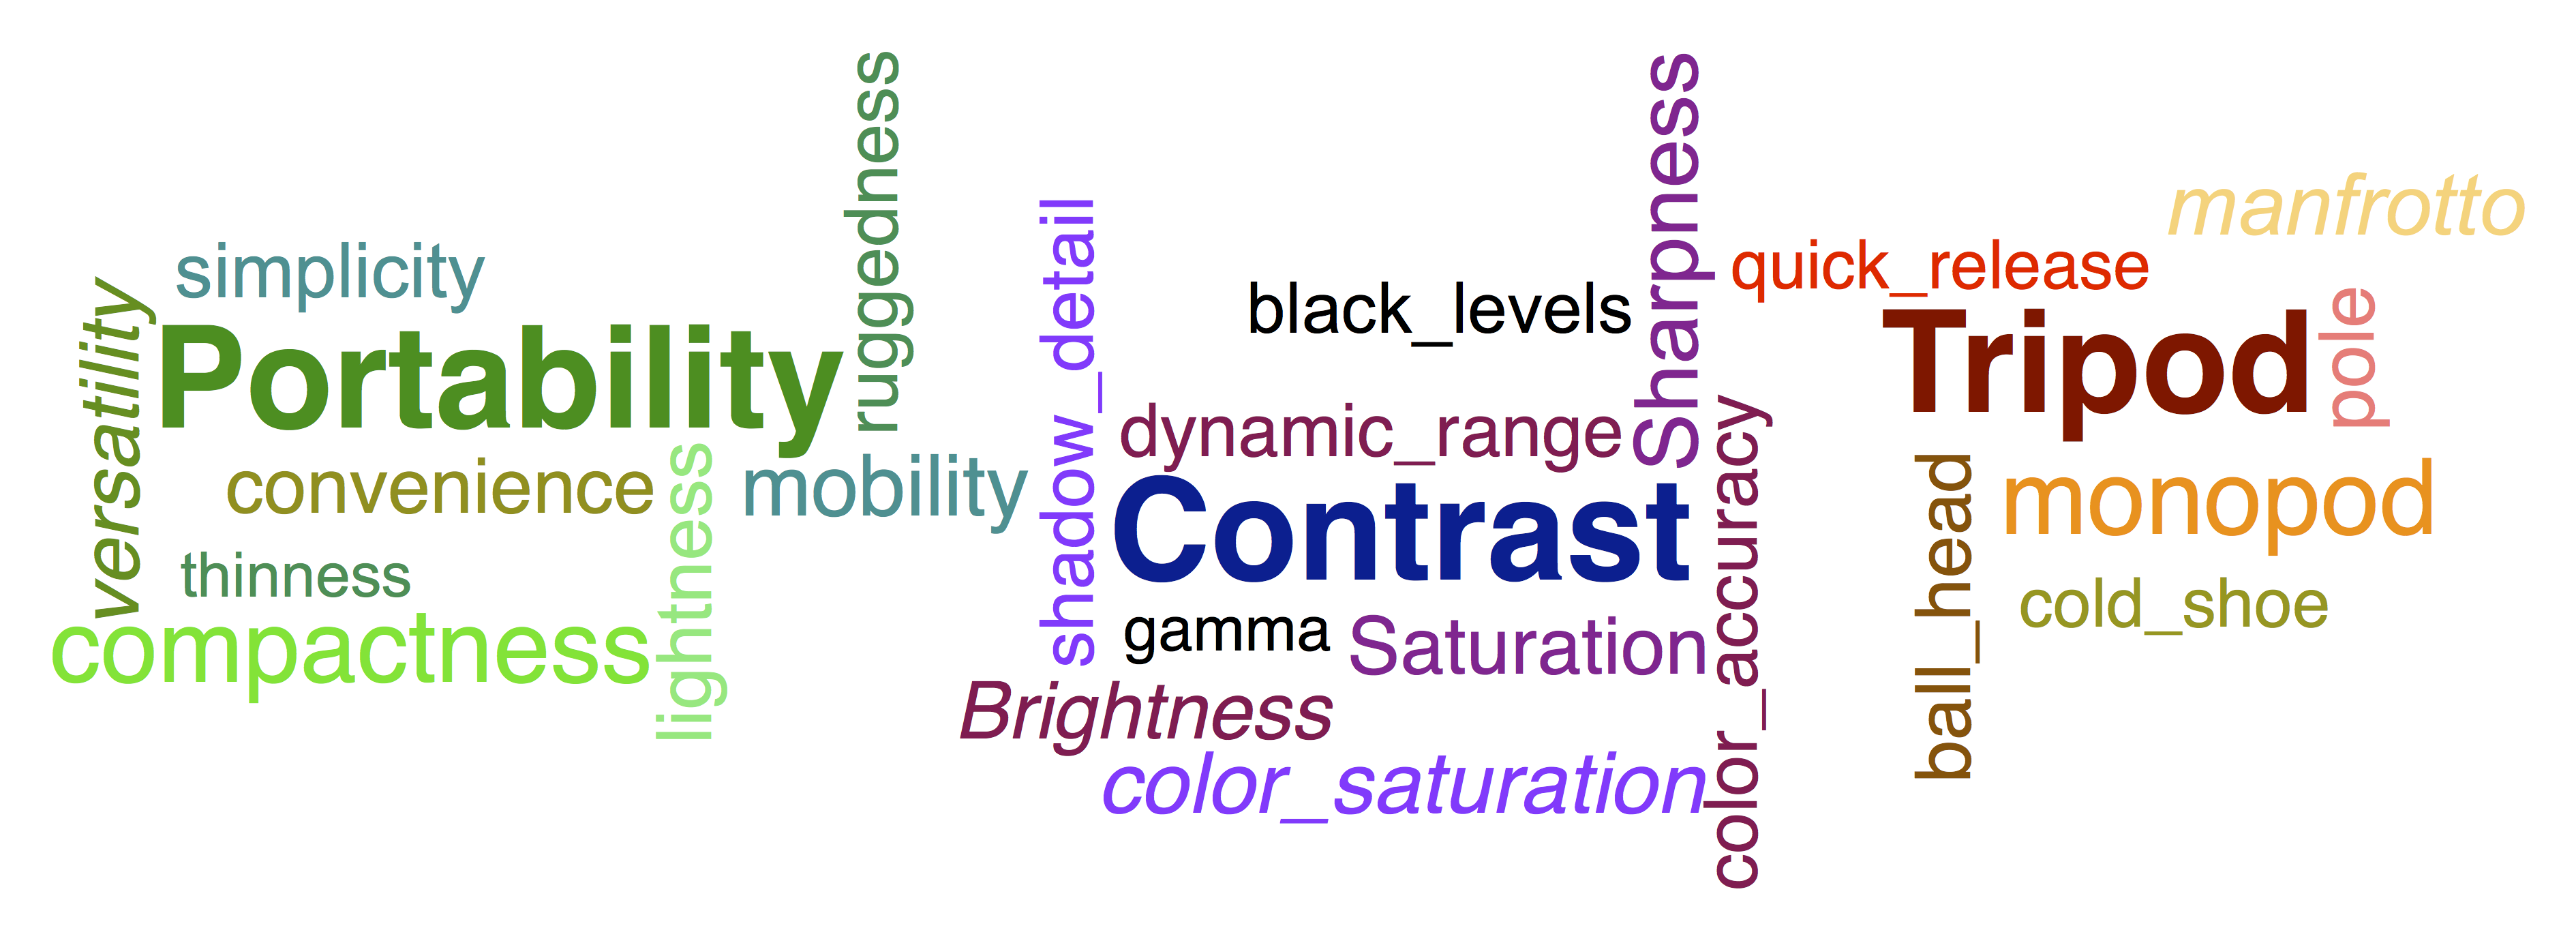
\includegraphics[width=.85\columnwidth]{Aspects_long.png}
\end{center}
\caption{Aspects.}
\label{aspectFig}
\end{figure}


\subsection{Qualitative evaluation of sentiment}

compare with google product reviews / cnet reviews

Error analysis
does not do comparative judgments.

My old computer was better...




\section{Conclusion}

conclusion







\subsubsection*{Acknowledgments}

We would like to acknowledge funding for computing resources provided by the Deep Social Learning Lab at Stanford.

\subsubsection*{References} % chronological. any citation style is acceptable, as long as it's consistent. Use APA

\small{

[1] Titov, I., \& McDonald, R. T. (2008). A Joint Model of Text and Aspect Ratings for Sentiment Summarization. In {\it ACL} (Vol. 8, pp. 308-316).

[2] Jo, Y., \& Oh, A. H. (2011). Aspect and sentiment unification model for online review analysis. In Proceedings of the fourth ACM international conference on Web search and data mining (pp. 815-824). ACM.

[3] Brody, S., \& Elhadad, N. (2010). An unsupervised aspect-sentiment model for online reviews. In {\it Human Language Technologies: The 2010 Annual Conference of the North American Chapter of the Association for Computational Linguistics} (pp. 804-812). Association for Computational Linguistics.

[4] Engonopoulos, N., Lazaridou, A., Paliouras, G., \& Chandrinos, K. (2011). ELS: a word-level method for entity-level sentiment analysis. In {\it Proceedings of the International Conference on Web Intelligence, Mining and Semantics}


[5] Moilanen, K., \& Pulman, S. (2009). Multi-entity Sentiment Scoring. In {\it Recent Advances in NLP} (pp. 258-263).


[6] Lakkaraju, H., Socher, R, \& Manning, C. (2014). Aspect Specific Sentiment Analysis using Hierarchical Deep Learning. {\it NIPS Workshop on Deep Learning and Representation Learning}

[7] Socher, R., Perelygin, A., Wu, J. Y., Chuang, J., Manning, C. D., Ng, A. Y., \& Potts, C. (2013). Recursive deep models for semantic compositionality over a sentiment treebank. In {\it Proceedings of the conference on Empirical Methods in Natural Language Processing (EMNLP)} (Vol. 1631, p. 1642).


%[8] Ghose, A., \& Ipeirotis, P. G. (2007). Designing novel review ranking systems: predicting the usefulness and impact of reviews. In {\it Proceedings of the Ninth international conference on Electronic commerce} (pp. 303-310). ACM.

%[9] Chen, P. Y., Dhanasobhon, S., \& Smith, M. D. (2008). All reviews are not created equal: The disaggregate impact of reviews and reviewers at Amazon.com. Available at SSRN: http://ssrn.com/abstract=918083 

%[10] Dai, W., Jin, G. Z., Lee, J., \& Luca, M. (2012). Optimal aggregation of consumer ratings: an application to Yelp.com (No. w18567). National Bureau of Economic Research. 


[8] McAuley, J., Targett, C., Shi, J., \& van den Hengel, A. (2015). Image-based recommendations on styles and substitutes. {\it ACM Special Interest Group on Information Retrieval (SIGIR)}

[9] Bird, Steven, Loper, E. and Klein, E. (2009). Natural Language Processing with Python. O’Reilly Media Inc.



%% this paper isn't that relevant. it's an evaluation system.
%[2] Ward, C. B., Choi, Y., Skiena, S., \& Xavier, E. C. (2011). Empath: A framework for evaluating entity-level sentiment analysis. In {\it Emerging Technologies for a Smarter World (CEWIT), 2011 8th International Conference \& Expo}. (pp. 1-6). IEEE.


%
%Wang, H., Lu, Y., & Zhai, C. (2010, July). Latent aspect rating analysis on review text data: a rating regression approach. In Proceedings of the 16th ACM SIGKDD international conference on Knowledge discovery and data mining (pp. 783-792). ACM.
%
%Yatani, K., Novati, M., Trusty, A., & Truong, K. N. (2011, May). Review spotlight: a user interface for summarizing user-generated reviews using adjective-noun word pairs. In Proceedings of the SIGCHI Conference on Human Factors in Computing Systems (pp. 1541-1550). ACM.



}

\end{document}
